A crucial component of any particle physics experiment is the magnet system, which enables the bending of charged particle trajectories allowing their momentum and charge to be measured. In ATLAS, this is achieved through a combination of two types of superconducting magnet systems, solenoidal and toroidal.

The main elements of the ATLAS magnet system include the central solenoid~\cite{atlas_central_solenoid}, the barrel toroid~\cite{atlas_barrel_toroid}, and the end-cap toroids~\cite{atlas_endcap_toroid}. An illustration of the magnetic system can be seen in Figure~\ref{fig:atlas_magnetic_field_map}. The central solenoid surrounds the ID, measuring 5.8 meters in length and 2.56 meters in diameter, and provides a uniform magnetic field of 2~T to the ID region.

\begin{figure}
    \centering
    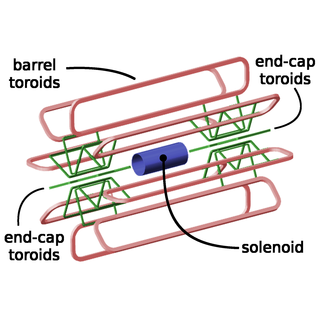
\includegraphics[width=0.8\textwidth]{figures/atlas/atlas_magnetic_system_illustration.png}
    \caption{A rough schematic of the ATLAS magnetic system. In the center is the superconducting solenoid for the ID, followed by the MS magnet system that consists of eight large barrel toroids and two large end-cap toroids. Taken from~\cite{atlas_magnetic_system_illustration}}\label{fig:atlas_magnet_system}
\end{figure}

The barrel and end-cap toroids, in contrast, generate a non-uniform magnetic field that can reach up to 3.5~T, which is essential for accurately measuring the momentum of muons. The barrel toroid is composed of eight coils and is the largest toroidal magnet ever constructed, with a total length of 25.3 meters. On both sides of the barrel are the two end-cap toroids, each with a diameter of 10.7 meters.

During operation, all of these magnets are cooled to about 4.5 K, in order to provide the necessary strong magnetic fields that are required for the experiment.
The magnetic field configuration in the transverse plane and longitudinal plane can be seen in Figure~\ref{fig:atlas_magnetic_field_map}.

\begin{figure}[pht]
    \centering
    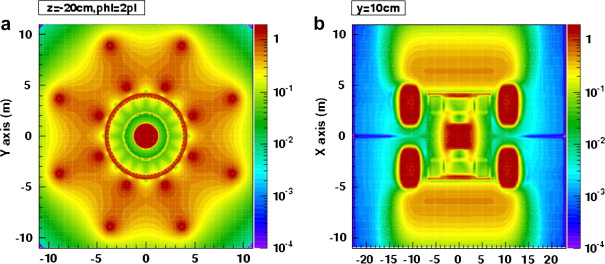
\includegraphics[width=0.8\textwidth]{figures/atlas/atlas_magnetic_field.jpg}
    \caption{A heatmap of the magnetic field strength in different cross section views of ATLAS\@. On the left, this shows the magnetic field in the transverse plane, hence no end-cap toroidal field. The figure on the right shows the magnetic field strength in the longitudinal plane. Taken from~\cite{atlas_magnetic_field_map}}\label{fig:atlas_magnetic_field_map}
\end{figure}